\documentclass[a4paper,10pt]{article}

%% Packages
\usepackage{epigraph}
\usepackage{fancyhdr}
\usepackage{geometry}
\usepackage{hyperref}
\usepackage{setspace}
\usepackage{tabularx}

\usepackage[pdftex]{graphicx}
\usepackage{wrapfig}

%% Headers
\pagestyle{fancy}

\fancyhead[RO,RE]{\it Curriculum Vitae}
\fancyfoot[LO,LE]{\it Noortje J. Venhuizen, PhD}

\renewcommand{\headrulewidth}{0.2pt}
\renewcommand{\footrulewidth}{0.2pt}

%% Font
\usepackage{tgpagella}
\usepackage[T1]{fontenc}
\linespread{1.25}

%% Spacing
%\onehalfspacing

%% Left column width
\def\leftcolwidth{.12\textwidth}

%% Vertical spacing
\def\tablevspace{10pt}


\begin{document}

%%%%%%%%%%%%%%%%%%%%%%%%%%%%%%%%%%%%%%%%%%%%%%%%%%%%%%%%%%%%%%%%%%%%%%%%%%
%% Name                                                                 %%
%%%%%%%%%%%%%%%%%%%%%%%%%%%%%%%%%%%%%%%%%%%%%%%%%%%%%%%%%%%%%%%%%%%%%%%%%%

\begin{flushright}
{\Huge Noortje J. Venhuizen, PhD}
\end{flushright}

%%%%%%%%%%%%%%%%%%%%%%%%%%%%%%%%%%%%%%%%%%%%%%%%%%%%%%%%%%%%%%%%%%%%%%%%%%
%% Personal Information                                                 %%
%%%%%%%%%%%%%%%%%%%%%%%%%%%%%%%%%%%%%%%%%%%%%%%%%%%%%%%%%%%%%%%%%%%%%%%%%%

\section*{Personal Information}

\begin{wrapfigure}{r}{0.5\textwidth}
  \begin{flushright}
  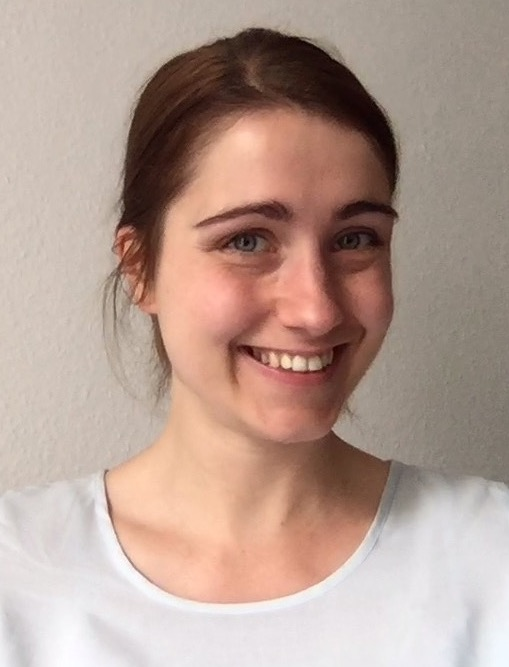
\includegraphics[width=0.3\textwidth]{noortje.jpg}
  \end{flushright}
\end{wrapfigure}

%% Name
\noindent
\begin{tabularx}{\textwidth}{ p{\leftcolwidth} X }
  Full name:      &         Noortje Joost Venhuizen\\
\end{tabularx}

\vspace{\tablevspace}

%% Birth and Nationality
\noindent
\begin{tabularx}{\textwidth}{ p{\leftcolwidth} X }
  Birthdate:   &         19--10--1986 (October 19th, 1986)\\
  Birthplace:  &         Groningen, The Netherlands\\
  Nationality: &         Dutch\\
  BSN:         &         199354261\\
\end{tabularx}

\vspace{\tablevspace}

%% E-mail address
\noindent
\begin{tabularx}{\textwidth}{ p{\leftcolwidth} X }
  E-mail:         
  &         \href{mailto:njvenhuizen@gmail.com}{njvenhuizen@gmail.com}\\
\end{tabularx}

\vspace{\tablevspace}

%% Personal homepage
\noindent
\begin{tabularx}{\textwidth}{ p{\leftcolwidth} X }
  Homepage:    &       \url{http://noortjejoost.github.io}
\end{tabularx}


%%%%%%%%%%%%%%%%%%%%%%%%%%%%%%%%%%%%%%%%%%%%%%%%%%%%%%%%%%%%%%%%%%%%%%%%%%
%% Degrees                                                              %%
%%%%%%%%%%%%%%%%%%%%%%%%%%%%%%%%%%%%%%%%%%%%%%%%%%%%%%%%%%%%%%%%%%%%%%%%%%

\section*{Degrees}

\noindent
\begin{tabularx}{\textwidth}{ p{\leftcolwidth} X }
  2011 -- 2015
  & \textbf{PhD degree in Computational Semantics}, 
    \textit{Center for Language and Cognition Groningen (CLCG)}, 
    \textit{University of Groningen}. Promotores: Prof. dr. J. Bos and Prof.
      dr. P. Hendriks.\\
  & \\
  & \textit{Dissertation}: `Projection in Discourse: A data-driven formal
      semantic analysis'; Jury: Prof. dr. N. M. Asher,
      Prof. dr. J. Hoeksema, and Prof. dr. R. A. van der Sandt; Opposition:
      Prof. dr. L. B. W. Geurts, Prof. dr. J. A. W. Kamp, dr. E. Maier, 
      and dr. H. W. Zeevat.
  \end{tabularx}

\vspace{\tablevspace}

%% MSc in Logic
\noindent
\begin{tabularx}{\textwidth}{ p{\leftcolwidth} X }
  2009 -- 2011  
  & \textbf{MSc degree in Logic}, Track: `Logic \& Language', 
    \textit{Institute for Logic, Language and Computation (ILLC)},
    \textit{University of Amsterdam}.\\
  & \\
  & \textit{Thesis}: `Negation in Questions'; Advisors: dr. F. Roelofsen and dr. G. Weidman Sassoon.
\end{tabularx}

\vspace{\tablevspace}

%% BA in Artificial Intelligence
\noindent
\begin{tabularx}{\textwidth}{ p{\leftcolwidth} X }
  2006 -- 2009  
  & \textbf{BSc degree in Artificial Intelligence 
    (\textit{cum laude}--highest possible distinction)}, 
    \textit{University of Utrecht}.\\
  & \\
  & \textit{Thesis}: `Donkey anaphora and Skolem functions'; Advisor: dr. Y. Winter.
\end{tabularx}

%%%%%%%%%%%%%%%%%%%%%%%%%%%%%%%%%%%%%%%%%%%%%%%%%%%%%%%%%%%%%%%%%%%%%%%%%%
%% Positions Held                                                       %%
%%%%%%%%%%%%%%%%%%%%%%%%%%%%%%%%%%%%%%%%%%%%%%%%%%%%%%%%%%%%%%%%%%%%%%%%%%

\section*{Positions Held}

\noindent
\begin{tabularx}{\textwidth}{ p{\leftcolwidth} X }
  2016 -- %11 MAR 2016 - 11 SEP 2016
  & \textbf{Postdoctoral researcher}, \textit{Universit\"at des Saarlandes,
      Saarbr\"ucken}.\\
\end{tabularx}

\vspace{\tablevspace}

\noindent
\begin{tabularx}{\textwidth}{ p{\leftcolwidth} X }
  2015 -- 2016 %OKT 2015-MAR 2016
  & \textbf{Postdoctoral researcher}, \textit{SFB 1102: Information Density and
      Linguistic Encoding, Project A1, Universit\"at des Saarlandes,
      Saarbr\"ucken}.\\
\end{tabularx}

\vspace{\tablevspace}

\noindent
\begin{tabularx}{\textwidth}{ p{\leftcolwidth} X }
  2015 %APR-SEP 2015
  & \textbf{Teaching position (Lehrauftrag)}, \textit{Universit\"at des
      Saarlandes, Saarbr\"ucken}.\\
\end{tabularx}

\vspace{\tablevspace}

\noindent
\begin{tabularx}{\textwidth}{ p{\leftcolwidth} X }
  2011 -- 2015 %1 SEP 2011 - 30 SEP 2015
  & \textbf{PhD candidate}, \textit{Center for Language and Cognition
      Groningen (CLCG), University of Groningen, Groningen}.\\
\end{tabularx}

\vspace{\tablevspace}

\noindent
\begin{tabularx}{\textwidth}{ p{\leftcolwidth} X }
  2010 -- 2011
  & \textbf{Various teaching assistantships}, \textit{Institute for Logic,
      Language and Information (ILLC), University of Amsterdam}. See
      `Teaching experience'.\\
\end{tabularx}

%%%%%%%%%%%%%%%%%%%%%%%%%%%%%%%%%%%%%%%%%%%%%%%%%%%%%%%%%%%%%%%%%%%%%%%%%%
%% Teaching Experience                                                  %%
%%%%%%%%%%%%%%%%%%%%%%%%%%%%%%%%%%%%%%%%%%%%%%%%%%%%%%%%%%%%%%%%%%%%%%%%%%

\section*{Teaching experience}

%% Semantic Theory
\noindent
\begin{tabularx}{\textwidth}{ p{\leftcolwidth} X }
  2016
  & \textbf{Semantic Theory (Teacher)}, \textit{Research Master Language
  Science and Technology (LST), Saarland University}.\\
\end{tabularx}

\vspace{\tablevspace}

%% FLST: Semantics
\noindent
\begin{tabularx}{\textwidth}{ p{\leftcolwidth} X }
  2016
  & \textbf{Foundations in Language Science and Technology: Semantics (Teacher)},
  \textit{Research Master Language
  Science and Technology (LST), Saarland University}.\\
\end{tabularx}

\vspace{\tablevspace}

%% Semantic Theory
\noindent
\begin{tabularx}{\textwidth}{ p{\leftcolwidth} X }
  2015
  & \textbf{Semantic Theory (Teacher)}, \textit{Research Master Language
  Science and Technology (LST), Saarland University}.\\
\end{tabularx}

\vspace{\tablevspace}

%% Guest Lecture
\noindent
\begin{tabularx}{\textwidth}{ p{\leftcolwidth} X }
  2014
  & \textbf{Linguistic Theory: Semantics (Guest Lecturer)}, 
    \textit{Research Master Linguistics, University of Groningen},
    Teacher: Prof. dr. P. Hendriks,
    Talk: `Discourse Representation Theory and its applications'.
\end{tabularx}

\vspace{\tablevspace}

%% Guest Lecture
\noindent
\begin{tabularx}{\textwidth}{ p{\leftcolwidth} X }
  2013
  & \textbf{Syntactic and Semantic Theory (Guest Lecturer)},
    \textit{Research Master Linguistics, University of Groningen},
    Teacher: Prof. dr. P. Hendriks,
    Talk: `Introducing DRT and PDRT'.
\end{tabularx}

\vspace{\tablevspace}

%% Textmanipulatie
\noindent
\begin{tabularx}{\textwidth}{ p{\leftcolwidth} X }
  2013
  & \textbf{Textmanipulation---UNIX tools (Teacher)}, 
    \textit{Bachelor Information Science, University of Groningen}.\\
\end{tabularx}

\vspace{\tablevspace}

\noindent
\begin{tabularx}{\textwidth}{ p{\leftcolwidth} X }
  2012
  & \textbf{Textmanipulation---UNIX tools (Teacher)}, 
    \textit{Bachelor Information Science, University of Groningen}.\\
\end{tabularx}

\vspace{\tablevspace}

%% TA Logic
\noindent
\begin{tabularx}{\textwidth}{ p{\leftcolwidth} X }
  2011
  & \textbf{Logic (Teaching assistant)}
    \textit{Bachelor Beta-Gamma, University of Amsterdam},
    Teacher: dr. J. Jaspars.
\end{tabularx}

\vspace{\tablevspace}

\noindent
\begin{tabularx}{\textwidth}{ p{\leftcolwidth} X }
  2010
  & \textbf{Logic (Teaching assistant)}
    \textit{Bachelor Beta-Gamma, University of Amsterdam},
    Teacher: dr. J. Jaspars.
\end{tabularx}

\vspace{\tablevspace}

%% TA Mathematical Logic
\noindent
\begin{tabularx}{\textwidth}{ p{\leftcolwidth} X }
  2010
  & \textbf{Introduction to Mathematical Logic (Teaching assistant)},
    \textit{Bachelor Mathematics, University of Amsterdam},
    Teacher: Prof. dr. Y. Venema.\\
\end{tabularx}

%%%%%%%%%%%%%%%%%%%%%%%%%%%%%%%%%%%%%%%%%%%%%%%%%%%%%%%%%%%%%%%%%%%%%%%%%%
%% Other Activities                                                     %%
%%%%%%%%%%%%%%%%%%%%%%%%%%%%%%%%%%%%%%%%%%%%%%%%%%%%%%%%%%%%%%%%%%%%%%%%%%

\section*{Other relevant activities}
%% Reviewer for: Proceeedings of *SEM 2012; TABU dag 2013; *SEM 2013, ...

%\begin{tabularx}{\textwidth}{ p{\leftcolwidth} X }
%  2014, 2015 
%       & \textbf{Participation in various Psycholinguistic conferences}:\\
%       & -- Architectures and Mechanisms for Language Processing (AMLaP) 20, 
%        September 3-6, 2014, \textit{University of Edinburgh, Scotland}\\
%       & -- BLIT/CELESE International Workshop on Neurocognitive Basis for Language, 
%        August 7, 2015, \textit{Waseda University, Tokyo, Japan}.\\
%\end{tabularx}

\vspace{\tablevspace}

% Organization `Open Dag op Locatie', Information Science, University of Groningen
\noindent
\begin{tabularx}{\textwidth}{ p{\leftcolwidth} X }
  2013 -- 2014
  & \textbf{Organisation of various information events for prospective students}, 
  \textit{BA Information Science}, \textit{University of Groningen}.\\
\end{tabularx}

\vspace{\tablevspace}

\noindent
\begin{tabularx}{\textwidth}{ p{\leftcolwidth} X }
  2013 & \textbf{Participation in LOT Summer School 2013} \textit{(Certificate acquired)}, June 17-28,
         \textit{Groningen, the Netherlands}.\\
       & -- {Masterclass Semantics and Pragmatics} (Prof. dr. L. B. W. Geurts)\\
       & -- {Quantity Implicatures} (Prof. dr. L. B. W. Geurts)\\
       & -- {Neurobiology of Language -- State of the Art} (Prof. dr. J. C. J. Hoeks)\\
\end{tabularx}

\vspace{\tablevspace}

%% Local organisation LOT summer school 2013
\noindent
\begin{tabularx}{\textwidth}{ p{\leftcolwidth} X }
  2013
  & \textbf{Member Local organisation LOT Summer School 2013},
    \textit{CLCG, University of Groningen}.\\
\end{tabularx}

\vspace{\tablevspace}

\noindent
\begin{tabularx}{\textwidth}{ p{\leftcolwidth} X }
  2012 & \textbf{Participation in LOT Summer School 2012} 
         \textit{(Certificate acquired)}, July 2-13,
         \textit{Utrecht, the Netherlands}.\\
       & -- {Masterclass Discourse Interpretation} (Prof. dr. A. Kehler)\\
       & -- {Reference and Coherence in Discourse} (Prof. dr. A. Kehler)\\
       & -- {Discourse and Cognition -- State of the Art} (Prof. dr. T. J. M. Sanders)\\
       & -- {Implicit Learning and Second Language Acquisition}
         (dr. P. Rebuschat)\\
\end{tabularx}

\vspace{\tablevspace}

%%Studentlid Faculteitsraad Geesteswetenschappen
\noindent
\begin{tabularx}{\textwidth}{ p{\leftcolwidth} X }
  2009 -- 2010
  & \textbf{Member Student's Council (Student-lid Faculteitsraad)},
    \textit{Faculty of Humanities, University of Utrecht}.\\
\end{tabularx}

\vspace{\tablevspace}

%% Surveilleren
%\noindent
%\begin{tabularx}{\textwidth}{ p{\leftcolwidth} X }
%  2008-2009
%  & \textbf{Exam invigilator}\\
%  & \textit{BV Topselect detacheringen, Utrecht}\\
%\end{tabularx}
%
%\vspace{\tablevspace}

%% Huiswerkassistent
\noindent
\begin{tabularx}{\textwidth}{ p{\leftcolwidth} X }
  2007 -- 2009
  & \textbf{Tutor/ homework assistant}, \textit{StudentsPlus, Utrecht},
  Subjects: Mathematics, Physics.
\end{tabularx}

\vspace{\tablevspace}

%% OC lid
\noindent
\begin{tabularx}{\textwidth}{ p{\leftcolwidth} X }
  2007 -- 2008
  & \textbf{Student member Education Committee (OC)},
    \textit{Bachelor Artificial Intelligence, University of Utrecht}.\\
\end{tabularx}

\vspace{\tablevspace}

\noindent
\begin{tabularx}{\textwidth}{ p{\leftcolwidth} X }
  2005 & \textbf{Curso de Lingua Portuguesa para Estrangeiros} 
         \textit{(Certificate acquired)}, ``Portuguese as a foreign language''
         (Annual course), \textit{Universidade de Coimbra, Portugal}.
\end{tabularx}


%\vspace{\tablevspace}

%%%%%%%%%%%%%%%%%%%%%%%%%%%%%%%%%%%%%%%%%%%%%%%%%%%%%%%%%%%%%%%%%%%%%%%%%%
%% Publications                                                         %%
%%%%%%%%%%%%%%%%%%%%%%%%%%%%%%%%%%%%%%%%%%%%%%%%%%%%%%%%%%%%%%%%%%%%%%%%%%

\section*{Publications}

\subsection*{In preparation}

\noindent
    \textbf{Venhuizen, N. J.}, Bos, J., Hendriks, P., and Brouwer, H.
    (under revision). Discourse Semantics with Information Structure.
    Manuscript under revision for \textit{Journal of Semantics}.\\
    \\
    Brouwer, H., Crocker, M. W., \textbf{Venhuizen, N. J.}, and Hoeks, J.C.J.
    (under revision). A Neurocomputational Model of the N400 and the P600 in
    Semantic Processing. Manuscript under revision for \textit{Cognitive Science}.\\
    \\
    \textbf{Venhuizen, N. J.}, Crocker, M. W., and Brouwer, H. 
    (in prep.). Modeling the Interaction between Linguistic Experience and
    World Knowledge in Online Surprisal. Manuscript in preparation.\\
    \\
    \textbf{Venhuizen, N. J.}, Bos, J., Hendriks, P., and Brouwer, H. 
    (in prep.). Predicting Information Status in Discourse. Manuscript in
    preparation.
    %\\
    %\textbf{Venhuizen, N. J.} and Brouwer, H. (in prep.). Computing Semantic
    %Structures: Implementing Projective Discourse Representation Theory using
    %Functional Programming. Textbook in preparation.

\subsection*{Refereed}

\noindent
    Bos, J., Basile, V., Evang, K., \textbf{Venhuizen, N.J.}, and Bjerva, J.
    (forthcoming 2016). The Groningen Meaning Bank. In Ide, N. and Pustejovsky, J.,
    editors, \textit{Handbook of Linguistic Annotation -- Part Two: Case
    studies}, Text, Speech and Language Technology. Springer.\\
    \\
    \textbf{Venhuizen, N.J.}, Bos, J., Hendriks, P., and Brouwer, H. (2014).
    How and Why Conventional Implicatures Project. In Todd Snider et al.
    (eds.), \textit{Proceedings of Semantics and Linguistic Theory (SALT) 24},
    63-83, New York, USA.\\
    \\
    \textbf{Venhuizen, N.J.}, Bos, J. and Brouwer, H. (2013). Parsimonious 
    Semantic Representations with Projection Pointers. In \textit{Proceedings
    of the 10th International Conference on Computational Semantics (IWCS 2013)
    -- Long papers}, Potsdam, Germany.\\
    \\
    \textbf{Venhuizen, N.J.}, Basile, V., Evang, K. and Bos, J. (2013).
    Gamification for Word Sense Labeling. In \textit{Proceedings of the 10th 
    International Conference on Computational Semantics (IWCS 2013) --
    Short papers}, Potsdam, Germany.\\
    \\
    Roelofsen, F., \textbf{Venhuizen, N.J.} and Weidman Sassoon, G. (2013).
    Positive and negative polar questions in discourse. In \textit{Proceedings of
    Sinn und Bedeutung} 17, Paris, France.\\
    \\
    Basile, V., Bos, J., Evang, K. and \textbf{Venhuizen, N.J.} (2012). UGroningen:
    Negation detection with Discourse Representation Structures. In
    \textit{Proceedings of the First Joint Conference on Lexical and Computational
    Semantics (*SEM'12)}, Montr\'eal, Canada.\\
    \\
    Basile, V., Bos, J., Evang, K. and \textbf{Venhuizen, N.J.} (2012). Developing
    a large semantically annotated corpus. In \textit{Proceedings of the 8th
    International Conference on Language Resources and Evaluation (LREC'12)},
    Istanbul, Turkey.\\
    \\
    Basile, V., Bos, J., Evang, K. and \textbf{Venhuizen, N.J.} (2012). A platform
    for collaborative semantic annotation. In \textit{Proceedings of the
    Demonstrations at the 13th Conference of the European Chapter of the
    Association for Computational Linguistics (EACL'12)}, Avignon, France.

\subsection*{Non-refereed}

\noindent
    \textbf{Venhuizen, N. J.} and Brouwer, H. (2014). PDRT-SANDBOX: An
    implementation of Projective Discourse Representation Theory. In Verena
    Rieser and Philippe Muller (eds.), \textit{Proceedings of the 18th
    Workshop on the Semantics and Pragmatics of Dialogue (SemDial-DialWatt
    2014)}, 249-251, September 1-3, Edinburgh, Scotland.

\subsection*{Theses}

\noindent
    \textbf{Venhuizen, N. J.} (2015). \textit{Projection in Discourse:
      A data-driven formal semantic analysis}. PhD thesis, University of
      Groningen, Groningen, the Netherlands.\\
    \\
    \textbf{Venhuizen, N. J.} (2011). \textit{Negation in Questions}.
      ILLC Publications, Master of Logic Thesis (MoL) Series: MoL-2011-06,
      University of Amsterdam, Amsterdam, the Netherlands.

%%%%%%%%%%%%%%%%%%%%%%%%%%%%%%%%%%%%%%%%%%%%%%%%%%%%%%%%%%%%%%%%%%%%%%%%%%
%% Talks and Posters                                                    %%
%%%%%%%%%%%%%%%%%%%%%%%%%%%%%%%%%%%%%%%%%%%%%%%%%%%%%%%%%%%%%%%%%%%%%%%%%%

\section*{Talks and Posters}

%\subsection*{Upcoming}
    
\subsection*{Invited talks}

\noindent
    \textbf{Venhuizen, N. J.} (2016). Projection in Discourse: A data-driven
    formal semantic analysis. Invited talk presented at the 5th Polymnie
    meeting, February 4-5, LORIA, Nancy, France.\\
    \\
    \textbf{Venhuizen, N. J.} (2015). Projective Discourse Representation
    Theory. Invited talk presented at the Semantics and Pragmatics
    Colloquium, December 8, Radboud University, Nijmegen, the Netherlands.

\subsection*{Conference talks}

\noindent
    Brouwer, H., \textbf{Venhuizen, N. J.}, and Crocker, M. W. (2016). The
    Electrophysiology of Language Comprehension: A Neurocomputational Model.
    Talk presented at the International Conference on Language and Perception,
    June 13-16, Trondheim, Norway.\\
    \\
    \textbf{Venhuizen, N. J.}, Brouwer, H., and Crocker, M. W. (2016). When the
    food arrives before the menu: Modeling Event-driven Surprisal in Language
    Comprehension. Talk presented at the Pre-CUNY Workshop on Events in
    Language and Cognition (ELC 2016), March 2, Gainesville, FL, USA.\\
    \\
    \textbf{Venhuizen, N. J.} (2015). Data-driven Formal Semantics. Talk
    presented at the Workshop Projection in Discourse: from formal to
    data-driven approaches, November 27, University of Groningen, Groningen,
    the Netherlands.\\
    \\
    \textbf{Venhuizen, N. J.} and Basile, V. (2015). Generating Genitive
    Alternation using Projective Discourse Representation Theory.
    Talk presented at the 36th TABU Dag, June 4-5, Groningen, the Netherlands.\\
    \\
    \textbf{Venhuizen, N. J.}, Bos, J., Hendriks, P., and Brouwer, H. (2015). 
    Differentiating projection phenomena in a unified semantic framework.
    Talk presented at the workshop Redrawing Pragmasemantic Borders,
    March 19, Groningen, the Netherlands.\\
    \\
    \textbf{Venhuizen, N. J.}, Bos, J., Hendriks, P., and Brouwer, H. (2015). 
    Differentiating projection phenomena in a unified semantic framework.
    Talk presented at the department of Computational Linguistics and Phonetics,
    Universit{\"a}t des Saarlandes, March 5, Saarbr{\"u}cken, Germany.\\
    \\
    \textbf{Venhuizen, N. J.} and Brouwer, H. (2014). Harnessing Projection: A Formal
    Implementation of Projective Discourse Representation Theory. Talk
    presented at the 24rd Meeting of Computational Linguistics in the
    Netherlands (CLIN 2014), January 17, Leiden, The Netherlands.\\
    \\
    \textbf{Venhuizen, N.J.} (2013). Projection Phenomena in Discourse: Toward
    a formal and computational analysis. Talk
    presented in the masterclass on Semantics and Pragmatics (by Prof. dr. Bart
    Geurts), LOT Summer School 2013, June 19, Groningen, the Netherlands.\\
    \\
    \textbf{Venhuizen, N.J.} (2013). Factive presuppositions in discourse:
    Towards a formal analysis in PDRT. Talk presented at the 34th TABU Dag,
    June 13-14, Groningen, the Netherlands.\\
    \\
    \textbf{Venhuizen, N.J.}, Bos, J., and Brouwer, H. (2013). Parsimonious 
    Semantic Representations with Projection Pointers. Talk presented at
    the 10th International Conference on Computational Semantics (IWCS 2013),
    March 19-22, Potsdam, Germany.\\
    \\
    Roelofsen, F., \textbf{Venhuizen, N.J.}, and Weidman Sassoon, G. (2013).
    Positive and negative polar questions in discourse. Talk presented at
    Sinn und Bedeutung 17, September 8-10, Paris, France.\\
    \\
    \textbf{Venhuizen, N.J.} (2012). Projection Phenomena in Discourse. Talk
    presented in the masterclass on Discourse Interpretation (by Prof. dr.
    Andrew Kehler), LOT Summer School 2012, July 4, Utrecht, the Netherlands.\\
    \\
    Basile, V., Bos, J., Evang, K., and \textbf{Venhuizen, N.J.} (2012).
    UGroningen: Negation detection with Discourse Representation Structures.
    Talk presented in the Shared Task session of the First Joint Conference
    on Lexical and Computational Semantics (*SEM'12), June 7-8, Montr{\'e}al,
    Canada.\\
    \\
    Basile, V., Bos, J., Evang, K., and \textbf{Venhuizen, N.J.} (2012).
    Developing a large semantically annotated corpus. Talk presented at the
    8th International Conference on Language Resources and Evaluation
    (LREC'12), May 21-27, Istanbul, Turkey.\\
    \\
    Basile, V., Bos, J., Evang, K., and \textbf{Venhuizen, N.J.} (2012).
    A platform for collaborative semantic annotation. Talk presented at the
    Demonstrations session of the 13th Conference of the European Chapter of
    the Association for Computational Linguistics (EACL'12), April 23-27,
    Avignon, France.\\
    \\
    \textbf{Venhuizen, N.J.} (2012). Representing Projection Phenomena in
    DRT. Talk presented at the 22nd Meeting of Computational Linguistics in
    the Netherlands (CLIN 2012), January 20th, Tilburg, the Netherlands.

%% Posters
\subsection*{Posters}

\noindent
    Brouwer, H., \textbf{Venhuizen, N. J.} and Crocker, M. W. (2016). The
    Electrophysiology of Language Comprehension: A Neurocomputational Model.
    Poster presented at the Annual Meeting of the Cognitive Neuroscience
    Society (CNS 2016), April 2-5, New York, NY, USA.
    \\
    \textbf{Venhuizen, N. J.} and Brouwer, H. (2014). PDRT-SANDBOX:
    Implementing Projective Discourse Representation Theory. Poster
    presented at the 18th Workshop on the Semantics and Pragmatics of
    Dialogue (SemDial-DialWatt 2014), September 1-3, Edinburgh, Scotland.\\
    \\
    \textbf{Venhuizen, N. J.}, Bos, J., Hendriks, P., and Brouwer, H.
    (2014). How and Why Conventional Implicatures Project. Poster presented
    at the 24rd Semantics and Linguistic Theory Conference (SALT 24), May
    30-June 1, New York University, New York, USA.\\
    \\
    \textbf{Venhuizen, N.J.}, Basile, V., Evang, K. and Bos, J. (2013).
    Gamification for Word Sense Labeling. Poster presented at the 10th
    International Conference on Computational Semantics (IWCS'13), March
    19-22, Potsdam, Germany.\\
    \\
    Basile, V., Bos, J., Evang, K. and \textbf{Venhuizen, N.J.} (2013).
    Wordrobe: using Games with a Purpose for Linguistic Annotation. Poster
    presented at the 23rd Meeting of Computational Linguistics in the
    Netherlands (CLIN 2013), January 18, Enschede, the Netherlands.\\
    \\
    Basile, V., Bos, J., Evang, K. and \textbf{Venhuizen, N.J.} (2012).
    Creating a semantically annotated corpus based on Discourse
    Representation Theory. Poster presented at the 22nd Meeting of
    Computational Linguistics in the Netherlands (CLIN 2012), January 20,
    Tilburg, the Netherlands.


%%%%%%%%%%%%%%%%%%%%%%%%%%%%%%%%%%%%%%%%%%%%%%%%%%%%%%%%%%%%%%%%%%%%%%%%%%
%% Projects                                                             %%
%%%%%%%%%%%%%%%%%%%%%%%%%%%%%%%%%%%%%%%%%%%%%%%%%%%%%%%%%%%%%%%%%%%%%%%%%%

\section*{Projects}

\noindent
    \textbf{Groningen Meaning Bank} (In collaboration with J. Bos, V. Basile,
    K. Evang, and J. Bjerva). A large corpus of public domain texts annotated
    with semantic representations based on (Projective) Discourse Representation
    Theory. Website: \url{http://gmb.let.rug.nl}.\\
    \\
    \textbf{Wordrobe} (In collaboration with J. Bos, V. Basile, and
    K. Evang). A collection of linguistic `games with a purpose', including
    games on word senses, co-reference resolution, named entities, animacy, and
    information structure. Website: \url{http://wordrobe.housing.rug.nl}.

%%%%%%%%%%%%%%%%%%%%%%%%%%%%%%%%%%%%%%%%%%%%%%%%%%%%%%%%%%%%%%%%%%%%%%%%%%
%% Software                                                             %%
%%%%%%%%%%%%%%%%%%%%%%%%%%%%%%%%%%%%%%%%%%%%%%%%%%%%%%%%%%%%%%%%%%%%%%%%%%

\section*{Software}

\noindent
\textbf{PDRT-SANDBOX} (In collaboration with H. Brouwer). Haskell library that
    implements Discourse Representation Theory, and Projective Discourse
    Representation Theory. The library includes machinery for representing,
    building, and combining (unresolved) DRSs and PDRSs.
    Available at: \url{http://hbrouwer.github.io/pdrt-sandbox/} (under the
    Apache License, Version 2.0).

%%%%%%%%%%%%%%%%%%%%%%%%%%%%%%%%%%%%%%%%%%%%%%%%%%%%%%%%%%%%%%%%%%%%%%%%%%
%% Grants                                                               %%
%%%%%%%%%%%%%%%%%%%%%%%%%%%%%%%%%%%%%%%%%%%%%%%%%%%%%%%%%%%%%%%%%%%%%%%%%%

%%helaas...

%%%%%%%%%%%%%%%%%%%%%%%%%%%%%%%%%%%%%%%%%%%%%%%%%%%%%%%%%%%%%%%%%%%%%%%%%%
%% Honors and Awards                                                    %%
%%%%%%%%%%%%%%%%%%%%%%%%%%%%%%%%%%%%%%%%%%%%%%%%%%%%%%%%%%%%%%%%%%%%%%%%%%

%\section*{Honors and Awards}
%
%\noindent
%\begin{tabularx}{\textwidth}{ p{\leftcolwidth} X }
%  2009
%  & \textbf{BSc degree in Artificial Intelligence, \textit{cum laude}--highest possible distinction}, \textit{University of Utrecht}.\\
%\end{tabularx}

\end{document}
